\chapter{Tests}
This chapter includes test descriptions and results to validate the design against the requirements. First, the two directional antennas are tested to find their gain and ensure, that the transmitter and receiver have their maximum gain at the same frequency. Finally, the full test of the beam steering and transmitter locator is tested with the transmitter fixed at a known location in the test area.

\section{Test of Horn Antenna S-Parameters} \label{s:sparam_test}
The aim of this test is to test the reflection coefficient of the receiving antenna. The measurement will be used to choose the resonance frequency for the acceptance test.

\subsubsection{Equipment}
To perform the test the following equipment is needed:
\begin{itemize}
    \item Rohde \& Schwarz ZNA Vector Network Analyzer (\SI{10}{\mega\hertz}-\SI{43.5}{\giga\hertz})
    \item Rohde \& Schwarz ZN-Z54 Calibration Unit (\SI{9}{\kilo\hertz}-\SI{40}{\giga\hertz})
    \item \SI{50}{\ohm} antenna cable
\end{itemize}

\subsubsection{Procedure}
The test is performed once. The following explains the procedure for the test:
\begin{enumerate}
    \item Add power to VNA, connect antenna cable to VNA and Calibration unit.
    \item Make calibration test by choosing \textit{Cal $\rightarrow$ Quick Start Calibration $\rightarrow$ Apply} on the VNA.
    \item Disconnect antenna cable and reconnect to DUT.
    \item Set start and stop frequencies. 
    \item Ensure that VNA measures $S_{11}$-parameter by choosing \textit{Meas $\rightarrow$ $S_{11}$}.
\end{enumerate}
The receiver antenna is a horn antenna which is designed to work in the spectrum from \SI{4}{\giga\hertz} to \SI{7}{\giga\hertz}. The measurement is performed in the spectrum \SI{3}{\giga\hertz} to \SI{8}{\giga\hertz} in order to encaosulate the entire antenna frequency spectrum, with steps of \SI{25}{\mega\hertz}. 

\subsubsection{Result}
The following figure shows $S_{11}$ at the measured frequencies
\begin{figure}[H]
    \centering
    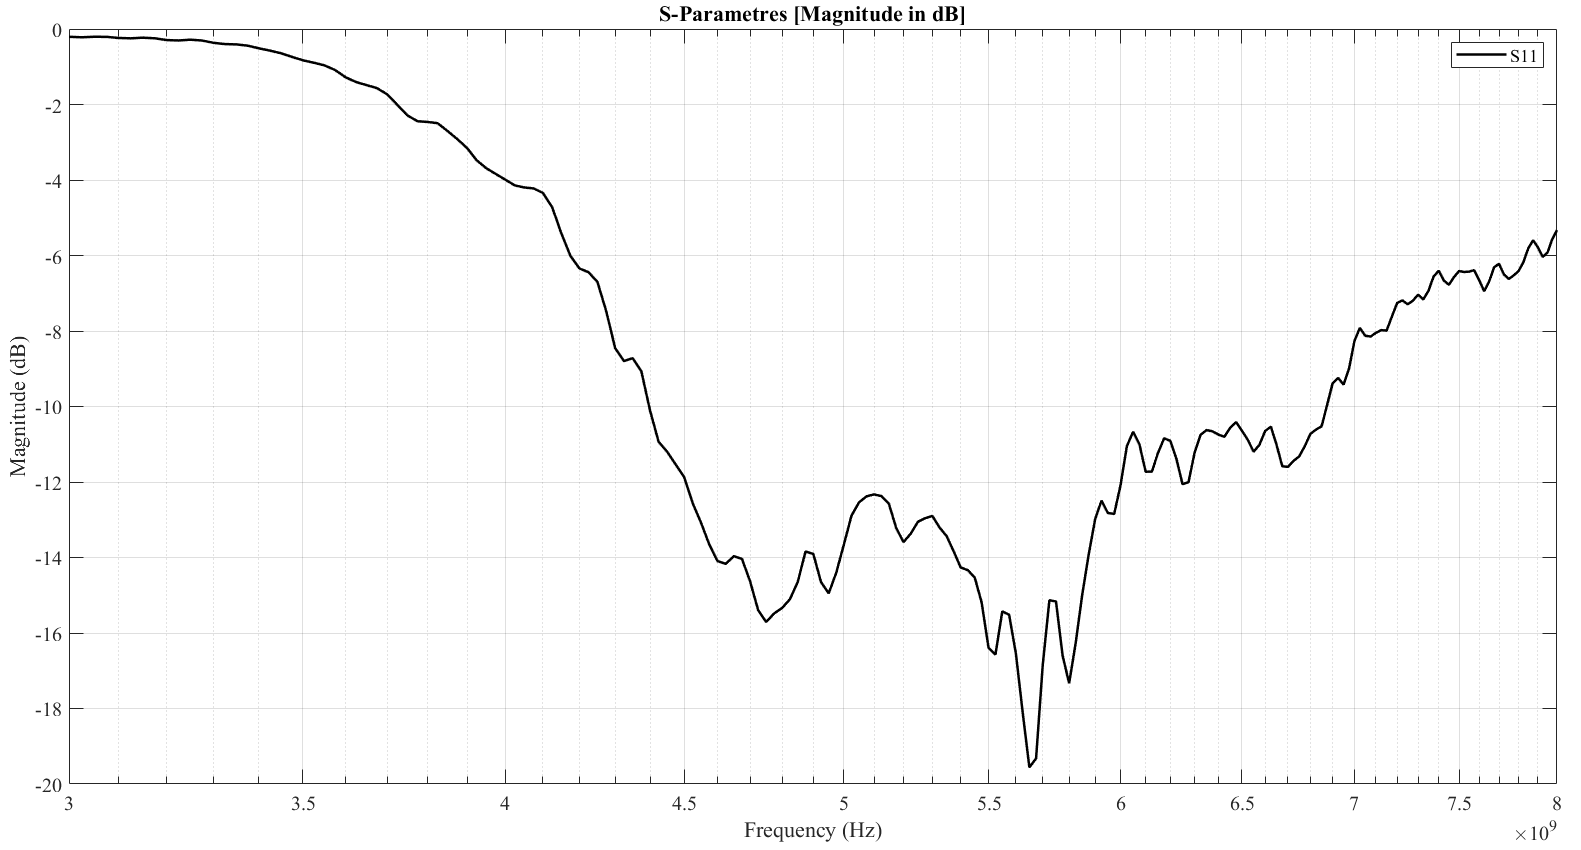
\includegraphics[width=1\textwidth]{figures/s11_meas.png}
    \caption{Measured $S_{11}$-parameter from \SI{3}{\giga\hertz} to \SI{8}{\giga\hertz}.} \label{fig:s11_meas}
\end{figure}
It can be seen that the antenna has a maximum $S_{11}$ magnitude of \SI{-19.56}{\decibel} at \SI{5.65}{\giga\hertz}. This gives a reflection coefficient of $\Gamma = 10^{-19.56/20} = 0.11$. Almost \SI{1}{\giga\hertz} away at \SI{4.75}{\giga\hertz} the magnitude of $S_{11}$ is \SI{-15.71}{\decibel} which equals a reflection coefficient of $\Gamma = 10^{-15.71/20} = 0.16$.

\section{Test of Horn Antenna Radiation Pattern} \label{s:rad_test}
The aim of this test is to know the directiveness of the receiving antenna. The measurement is used in the evaluation of the angle step of the turntable.

\subsubsection{Equipment}
The test is performed in the anechoic chamber at Aalborg University with the provided setup equipment at the site. This includes
\begin{itemize}
    \item Computer with relevant \textit{MVG software}
    \item \textit{MVG StarMIMO} in anechoic chamber
\end{itemize}
The \textit{MVG StarMIMO} has a measurement bandwidth of \SI{400}{\mega\hertz} to \SI{6}{\giga\hertz}. As seen in the results in the test of S-parameters in section \ref{s:sparam_test} the maximum reflection coefficient magnitude is at \SI{5.65}{\giga\hertz}, therefore the step size of frequency spectrum for the radiation characteristics measurement is chosen to be \SI{0.05}{\giga\hertz}.

\subsubsection{Procedure}
The following explains the procedure for the test:
\begin{enumerate}
    \item Measure known antenna \textit{(MVG SH800)} with known radiation characteristics. Use for gain reference.
    \item Secure DUT to test platform.
    \item Perform automated test by activating the measurement equipment outside the chamber.
\end{enumerate}
Since the antenna is not designed for use below \SI{4}{\giga\hertz}, this is set as the start frequency. The measurement equipment cannot measure above \SI{6}{\giga\hertz}, therefore this is the end frequency. The StarMIMO measures at angles of \SI{15}{\degree} in both planes.

\subsubsection{Result}
The data collected is imported into \textit{Matlab} for visualization. The figure \ref{fig:horn_elevation} shows the elevation plane of the measured horn antenna in the anechoic chamber. The red line shows the radiation pattern for the horn antenna at $f=\SI{4.75}{\giga\hertz}$. The blue line shows the radiation pattern for the horn antenna at $f=\SI{5.65}{\giga\hertz}$. The antenna has a higher gain at $f=\SI{5.65}{\giga\hertz}$ of \SI{12.99}{\decibel}, whereas at $f=\SI{4.75}{\giga\hertz}$ the highest gain is \SI{11.41}{\decibel}. The \SI{3}{\decibel}-bandwidths are also plotted at \SI{19}{\degree} for $f=\SI{5.65}{\giga\hertz}$ and at \SI{22.5}{\degree} for $f=\SI{4.75}{\giga\hertz}$.
\begin{figure}[H]
    \centering
    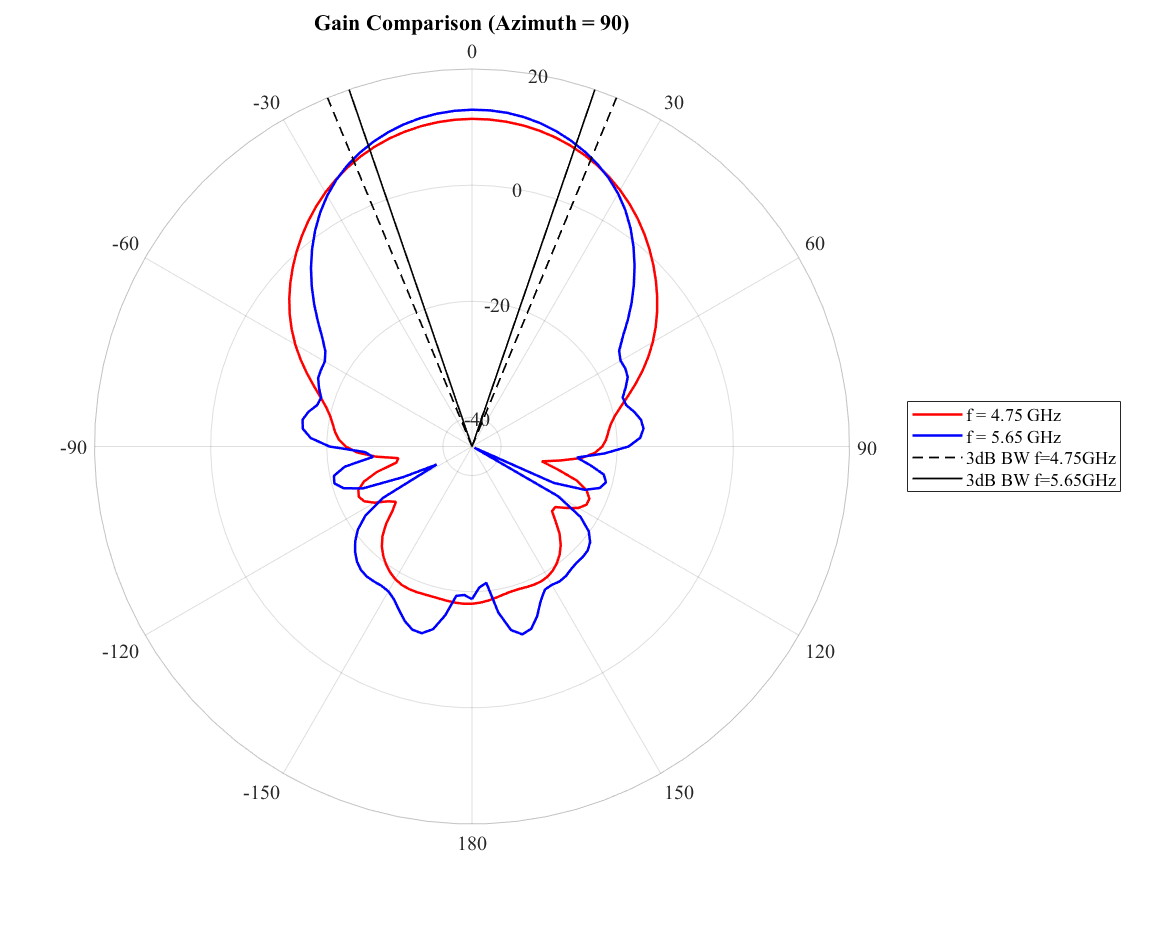
\includegraphics[width=1\textwidth]{figures/horn_elevation.png}
    \caption{Measured gain in the farfield at \SI{4.75}{\giga\hertz} and \SI{5.65}{\giga\hertz} (elevation plane).} 
    \label{fig:horn_elevation}
\end{figure}

The figure \ref{fig:horn_azimuth} below shows the azimuth plane of the horn antenna as measured in the anechoic chamber. The red line shows the gain for the antenna at $f=\SI{4.75}{\giga\hertz}$ and the blue line shows the gain for the antenna at $f=\SI{5.65}{\giga\hertz}$. The maximum gain is \SI{12.99}{\decibel} at \SI{0}{\degree}. 
\begin{figure}[H]
    \centering
    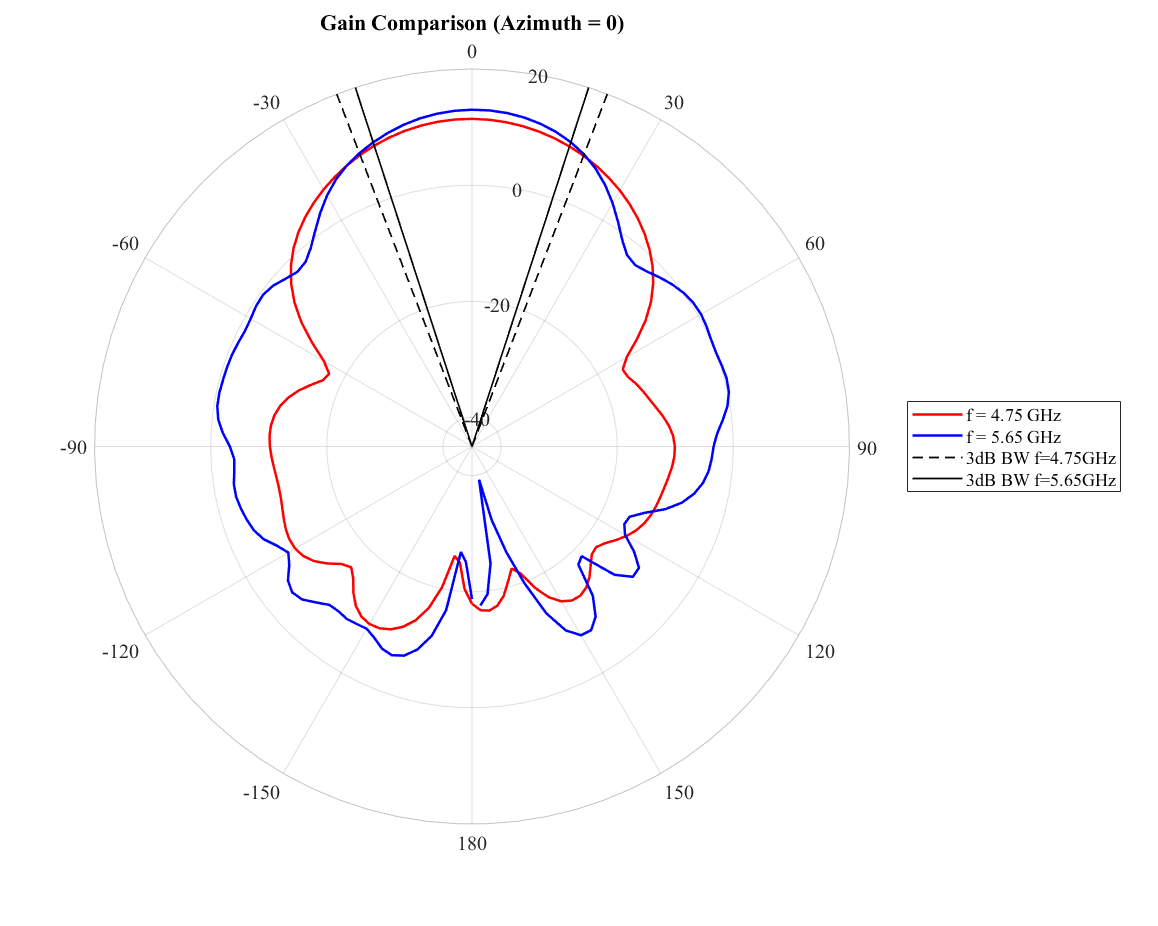
\includegraphics[width=1\textwidth]{figures/horn_azimuth.png}
    \caption{Measured gain in the farfield at \SI{4.75}{\giga\hertz} and \SI{5.65}{\giga\hertz} (azimuth plane).} 
    \label{fig:horn_azimuth}
\end{figure}

Simultaneously the maximum gain of the antenna over the frequency spectrum at any measured angle was measured as seen on the figure \ref{fig:gain_meas}. The measurement shows that the gain, generally, increases as the frequency increases.
\begin{figure}[H]
    \centering
    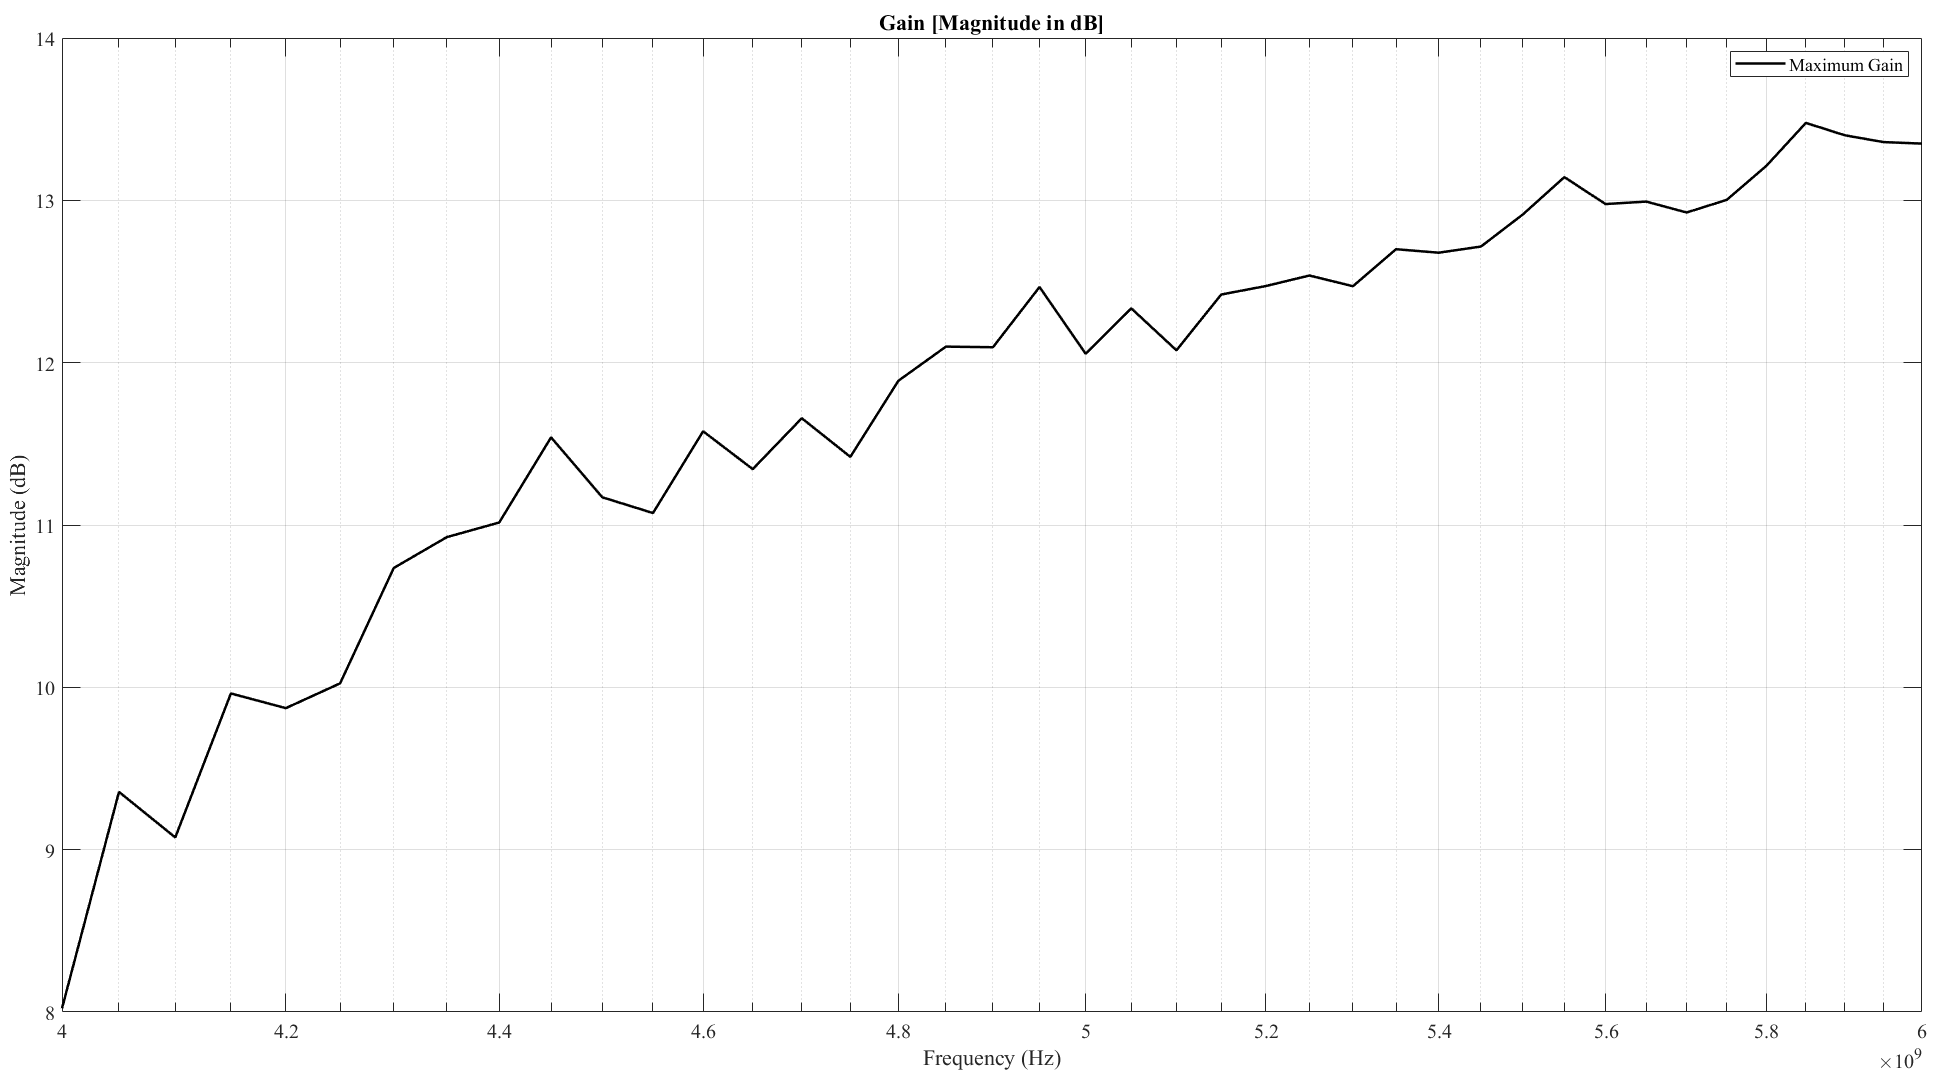
\includegraphics[width=1\textwidth]{figures/gain_meas.png}
    \caption{Measured maximum gain at any measured angle in the frequency spectrum from \SI{4}{\giga\hertz} to \SI{6}{\giga\hertz}.} \label{fig:gain_meas}
\end{figure}

\section{Accept Test}
The aim of this test is to test the full function of the developed product. The test must show that the receiver antenna on the turntable is able to scan the test area and measure the received power at fixed angles, before selection the location with the maximum received power and focusing its beam on that location. The test also contains test of intruder detection. In these scenarios the line-of-sight between the transmitter and receiver antennas is broken by an object. 

\subsubsection{Equipment}
To perform the test, the following equipment is needed:

\begin{itemize}
    \item HEAD Acoustics Remote-operated Turntable, model HRT I 6498, with \SI{24}{\volt} DC \SI{60}{W} power supply
    \item D-sub 9-pin to USB-A cable to connect turntable to PC
    \item PC with one USB-A port and one LAN port
    \item Rohde \& Schwarz ZVB 8 Vector Network Analyzer
    \item Network cable (8-pin RJ-45 connector) to connect VNA to PC
    \item Two identical horn antennas with dimensions as seen on figure \ref{fig:horn_design} in section \ref{s:ant_design}
    \item Two \SI{50}{\ohm} antenna cables
\end{itemize}

Moreover, the test must be performed in a controlled environment in order to ensure that the turntable and VNA can function optimally. The temperature must not be below \SI{5}{\celsius} or above \SI{40}{\celsius} with a relative humidity in the range \SI{20}{\percent} - \SI{80}{\percent}~\cite{hrt_i_data_sheet}\cite{vna_data_sheet_spec}.

\subsubsection{Test Execution}
The following steps outline how to perform the test:

\begin{enumerate}
    \item Power ZVB8 and HRT I. 
    \item Calibrate ZVB8 with calibration unit.
    \item Connect Windows PC to ZVB8 and HRT I.
    \item Connect transmitter antenna to port 2 on ZVB8 with antenna cable. Set channel power level to \SI{10}{dBm}.
    \item Connect receiver antenna to port 1 on ZVB8 with antenna cable.
    \item Setup transmitter antenna to point towards receiver antenna creating a line-of-sight between the two antennas. 
    \item Mount the receiver antenna on HRT I.
    \item Load Python code on Windows PC and run control program.
\end{enumerate}

Repeat the test procedure for different setups; antennas pointing straight to each other with and without intruder person, with the antennas in either corner of a room with and without intruder table, and with the transmitter perpendicular to the receiver antenna. Figure \ref{fig:experiment-setup} shows a simple diagram of the test setup from a horizontal angle.

\begin{figure}[H]
    \centering
    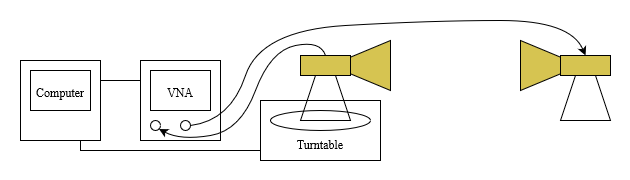
\includegraphics[width=0.8\textwidth]{figures/accept_test_setup.png}
    \caption{Setup for test of functionality of beam steering device.} \label{fig:experiment-setup}
\end{figure}

\subsubsection{Test Results}
\todo[inline,color=blue]{add table for test results and describe}


While the turntable is turning the cable connected to the horn antenna will move with it. This will affect the phase of the signal. However, since the purpose of the test is to measure magnitude, this error is will not effect the test result. 